\documentclass{beamer}

\usetheme{Montpellier}
\usepackage{tikz}

\definecolor{beamer@blendedblue}{rgb}{0.3,0.5,0.6}

\setbeamercolor{normal text}{fg=black, bg=white}
\setbeamercolor{alerted text}{fg=red}
\setbeamercolor{example text}{fg=green!50!blue}

\title{Virtual Reality for Sensor Data Analysis}
\subtitle{SW-Projekt SS 2017 Gruppe 5.1}
\author{Gero Birkh\"olzer \and Johannes Blank \and Alexej Gluschkow \\ \and Fabian Klopfer \and Lisa-Maria Mayer}
\date{Endpr\"asentation, 17. Juni 2017}



\addtobeamertemplate{frametitle}{}{%
\begin{tikzpicture}[remember picture,overlay]
\node[anchor=north east,yshift=2pt] at (current page.north east) {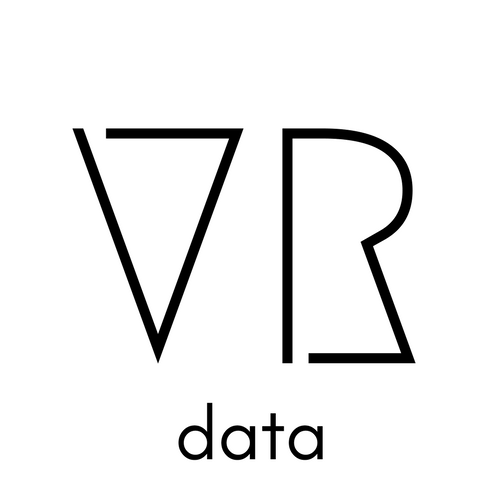
\includegraphics[height=0.8cm]{logo.png}};
\end{tikzpicture}}


\begin{document}


\frame{\titlepage}



\begin{frame}
  \frametitle{Inhalt}
  \tableofcontents%[hideallsubsections]
\end{frame}


\section{Use Case}



% ENGLISCH FREUNDE.... ENGLISCH!





\section{App \& WebVR}

\subsection{Android App}

\subsubsection{Overview}
\begin{frame} % !!!!! TODO Flow diagramm !!!!!!
\frametitle{Overview}
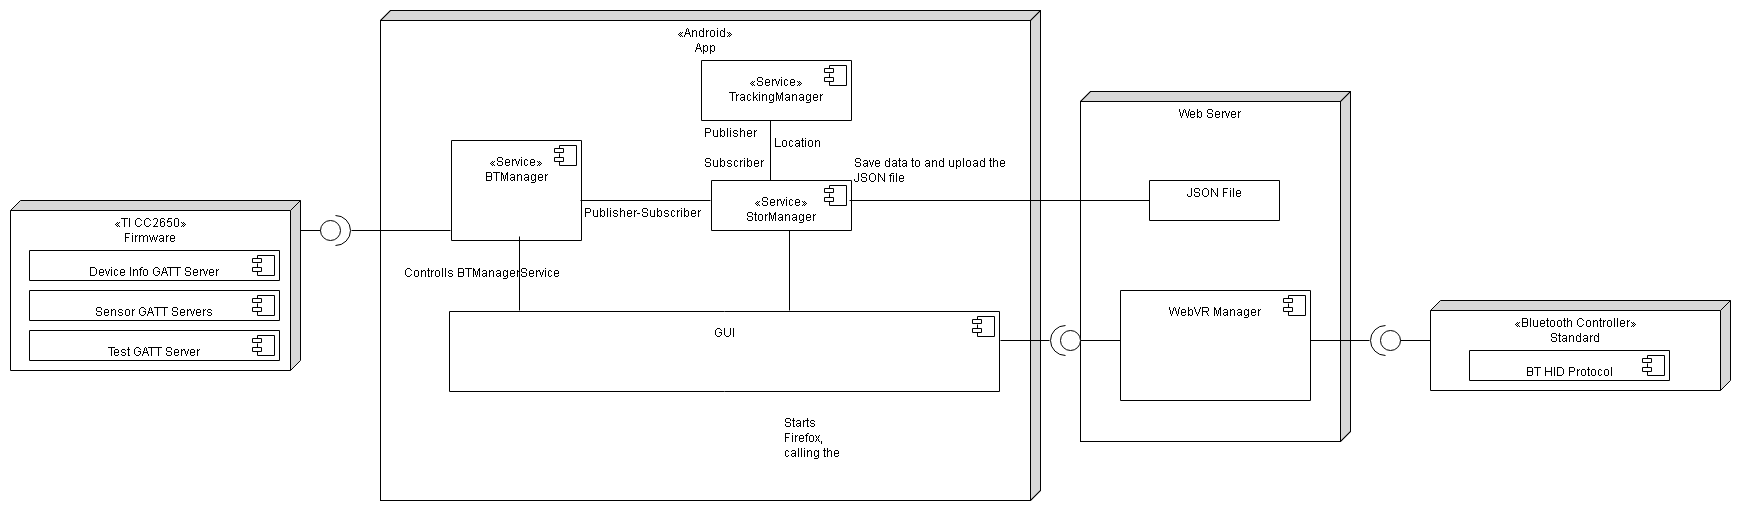
\includegraphics[width=\textwidth]{../doc/SDD/pics/composite_app.png}
\end{frame}

\subsubsection{Tracking}
\begin{frame}
\frametitle{Tracking}
\begin{itemize}
  	\item	Coarse tracking by GPS / Network Provider
 	\item 	Finer position tracking by RSSI trilateration using wifi access points:\\
			\begin{center}
			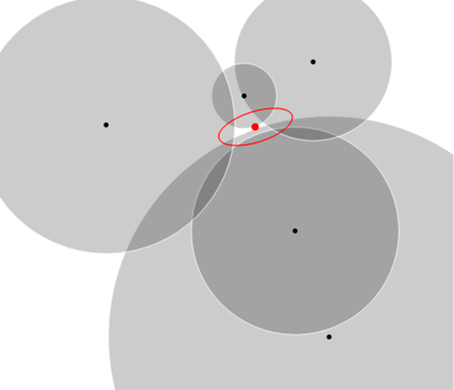
\includegraphics[scale=0.5]{trilateration.png}
			\end{center}

\end{itemize}
\end{frame}

\subsection{WebVR}
% TODO Maybe some pics ...
\begin{frame}
\frametitle{WebVR}
\begin{itemize}
  \item WebVR a javascript API to get VR into the browser \pause
%  \item Any VR headset or smartphone with Chrome or Firefox
  \item Basic 3D model of a gym \pause
  \item 2 different visualization possibilities
  \begin{itemize}
    \item datapoints
    \item plane
  \end{itemize}
\end{itemize}
\end{frame}

\begin{frame}
\frametitle{WebVR}
\begin{itemize}
  \item Interpolation of the Data \pause
  \item Using Inverse distance weighted (IDW) interpolation:
  \begin{center}
  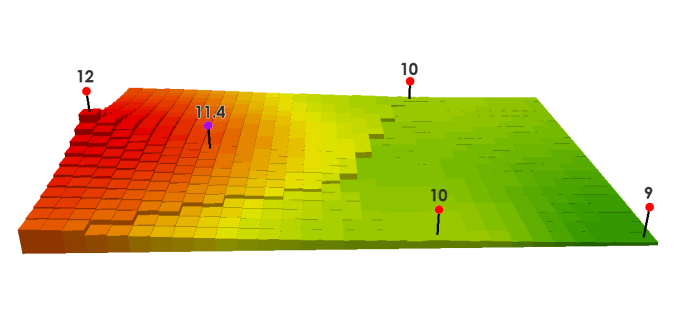
\includegraphics[scale=0.3]{IDW.png}
  \end{center}
  \pause
  \item Formula:
  $$
  u(x) = \frac{\sum_{i=1}^n w_i(x)u_i}{\sum_{i=1}^n w_i(x)}
  $$
\end{itemize}
\end{frame}

\section{live demonstration}
% Miracast
\begin{frame}
\frametitle{live demonstration using miracast or equal}

\end{frame}

\end{document}
